\documentclass[conference]{IEEEtran}

\usepackage{cite}
\usepackage{amsmath,amssymb,amsfonts}
\usepackage{algorithmic}
\usepackage{algorithm}
\usepackage{graphicx}
\usepackage{textcomp}
\usepackage{xcolor}
\usepackage{url}
\usepackage{array}
\usepackage{tikz}
\usepackage{pgfplots}
\pgfplotsset{compat=1.18}
\usetikzlibrary{arrows.meta,bending}

% Override IEEEtran's default \normalsize (10pt) affiliation font to \small (9pt).
% At 10pt, "Dept. of Computer Science and Engineering" is ~65mm wide per block;
% three blocks (195mm) exceed the 177.8mm text width and force a 2+1 wrap.
% At 9pt, each block is ~58mm; three blocks (174mm) fit in one row.
\makeatletter
\def\@IEEEauthorblockAstyle{\normalfont\small}
\makeatother

\begin{document}

\title{Design of a Dual-Controller System for Safe Autonomous Remediation in Stateful and Stateless Workloads}

\author{%
\IEEEauthorblockN{Pranav Negi}
\IEEEauthorblockA{\textit{Dept. of Computer Science and Engineering}\\
\textit{PES University}\\
Bengaluru, India\\
pes2ug23cs429@pesu.pes.edu}
\and
\IEEEauthorblockN{Reema Sarkar}
\IEEEauthorblockA{\textit{Dept. of Computer Science and Engineering}\\
\textit{PES University}\\
Bengaluru, India\\
pes2ug23cs471@pesu.pes.edu}
\and
\IEEEauthorblockN{Animesh Giri}
\IEEEauthorblockA{\textit{Dept. of Computer Science and Engineering}\\
\textit{PES University}\\
Bengaluru, India\\
animeshgiri@pesu.pes.edu}
}

\maketitle

\begin{abstract}
We present UnderCurrent, an eBPF-driven self-healing framework that separates stateless and stateful container workloads and uses finite-state-machine (FSM) gating to constrain recovery actions. Kernel-level events are collected through BCC-based eBPF probes and processed by a dual-track control plane: a threshold DAG for stateless workloads (Type~S) and an FSM-gated DAG with a WASM policy enforcement layer for stateful workloads (Type~F). Every decision cycle runs a real and a shadow path; divergences are tracked as an observable metric. Over 9,132 committed evaluation traces (4,564 stateful, 4,568 stateless), divergence between the real FSM path and the fresh-each-cycle shadow path occurs in 44 of 2,282 real stateful cycles ($M_2 = 0.0193$); the Type~S track produces zero divergences by construction. A controlled fault-injection campaign on \texttt{redis} ($N = 30$ episodes, all recovered) confirmed the FSM two-cycle recovery guarantee: mean MTTR 10.40\,s, $\sigma = 0.03$\,s, $\sigma/\mu < 0.3\%$. An ablation study on 2,282 real Type-F traces shows that removing FSM gating causes 44 premature checkpoint-and-restart dispatches, while a memoryless threshold policy misses all 44 legitimate checkpoint opportunities; the full FSM produces zero unsafe and zero missed dispatches. WASM sandbox overhead is 27\,$\mu$s per call (p99: 50\,$\mu$s) and shadow execution adds 8\,$\mu$s per cycle, both negligible at the 5\,s reconcile interval.
\end{abstract}

\begin{IEEEkeywords}
autonomic computing, eBPF, container remediation, finite state machines, shadow execution, safe remediation
\end{IEEEkeywords}

\section{Introduction}
\label{sec:intro}

Production deployments routinely mix workloads with different failure semantics. A crashed \texttt{nginx} worker: restart it. Done. A \texttt{postgres} instance showing sustained high-latency block~I/O is a harder problem---it requires a carefully sequenced flush-then-checkpoint procedure, and running that procedure too early may corrupt uncommitted transactions. Contemporary autonomic frameworks do not handle this difference well. They either apply one restart-or-reschedule policy across all containers~\cite{b1}, or hand the decision to human operators who cannot act at the sub-second cadence that eBPF (extended Berkeley Packet Filter) observability makes possible~\cite{b6}.

The difficulty is not signal collection. eBPF has made per-process kernel telemetry cheap, always-on, and low-overhead~\cite{b6}. The problem is decision safety. Autonomous remediation of stateful workloads requires three mechanisms operating together: an audit phase before any checkpoint operation (formal sequencing); blocking of irreversible actions until sequencing constraints are satisfied (reversibility enforcement); and per-cycle measurement of whether accumulated FSM state is changing decisions relative to what a memoryless policy would produce (behavioural observability).

The dual-track control plane described here addresses all three. Contributions:
\begin{enumerate}
\item A dual-track architecture running Type~S (stateless) and Type~F (stateful) pipelines on a shared eBPF event bus, with independent confidence scoring and sliding-window state stores per track (Section~\ref{sec:arch}).
\item A five-state FSM for Type~F that enforces action sequencing and irreversibility constraints separately from the confidence DAG, backed by a policy layer that gates actions at the execution boundary (Section~\ref{sec:typef}).
\item A real/shadow execution model that runs every reconcile cycle twice---once on the live FSM, once on a fresh throwaway---and logs divergence as a first-class metric (Section~\ref{sec:arch}).
\item A four-metric behavioural evaluation---divergence rate (M2), MTTR (M3), reversibility ratio (M4), and FSM-gated suppression rate (M6)---supplemented by two schema validation checks (M1, M5), with results collected using the deployed control plane on real Docker containers; the committed \texttt{data/phase2/} trace corpus was collected in simulation-event mode (Section~\ref{sec:eval}).
\item A decision-policy ablation on 2,282 real Type-F traces showing that FSM gating is strictly necessary: without it, 44 of 88 C\&R dispatches are premature; without state accumulation, all 44 legitimate C\&R opportunities are missed (Section~\ref{sec:ablation}).
\end{enumerate}

\section{Background and Related Work}
\label{sec:background}

\textbf{Autonomic computing and MAPE-K.} Kephart and Chess~\cite{b8} established the MAPE-K (Monitor-Analyse-Plan-Execute over a shared Knowledge base) loop as the standard architecture for self-managing systems. The design here maps onto it directly: eBPF probes cover Monitor, per-track confidence scorers cover Analyse, the FSM-gated DAG is Plan, and the action executor is Execute. Plan is split into two independent branches sharing a common event bus.

\textbf{Kubernetes operators and HPA/VPA.} Kubernetes Operators~\cite{b1} and Pod Autoscalers manage resources declaratively, but remediation stays limited to pod restarts and replica scaling. Neither operates at the I/O-path signal level, and neither enforces sequencing constraints during active I/O---precisely where stateful workload risk materialises.

\textbf{Chaos engineering.} Basiri et al.~\cite{b3} formalise chaos engineering as the practice of injecting controlled faults to reveal systemic weaknesses. The fault injection used here (§\ref{sec:m3}) applies the same philosophy at the signal level: synthetic \texttt{blk\_io\_latency} events exercise the full FSM recovery path without requiring a multi-node cluster. UnderCurrent complements chaos engineering by providing the automated recovery layer that chaos experiments are intended to stress-test.

\textbf{eBPF observability.} BCC (BPF Compiler Collection)~\cite{b6} makes kernel-level probes cheap enough to run continuously without user-space instrumentation. The implementation attaches kprobes on \texttt{blk\_account\_io\_start/done}, kretprobes on \texttt{vfs\_write/read}, and tracepoints on \texttt{mount} and \texttt{umount} syscalls---direct I/O and filesystem visibility at the kernel level, requiring no application modification.

\textbf{Checkpoint/restore and stateful recovery.} CRIU~\cite{b2} provides live process checkpointing via \texttt{/proc} and Linux namespaces. The \texttt{checkpoint\_and\_restart} action relies on CRIU to create memory snapshots before recovery; the FSM sequencing guarantee ensures this action is only dispatched after a full audit cycle, reducing the risk of checkpointing during an active transaction.

\textbf{Formal methods and shadow execution.} TLA+~\cite{b9} provides formal verification of state-machine properties at design time; the FSM enforces those transition constraints at runtime through executable guards. The shadow path follows Fowler's dark-launch pattern~\cite{b5}: every cycle runs on both the live FSM and a fresh throwaway, with divergence recorded as metric M2. The policy enforcement layer gates actions at the execution boundary using a sandboxed WebAssembly module~\cite{b4}.

\section{System Architecture}
\label{sec:arch}

\subsection{Overview}

Fig.~\ref{fig:arch} shows the full pipeline. Type~S and Type~F run as parallel threads sharing a common eBPF probe infrastructure. The pipeline is the same for both: kernel probes $\rightarrow$ per-track perf buffer $\rightarrow$ comm-filtered listener thread $\rightarrow$ sliding-window StateStore $\rightarrow$ confidence scorer $\rightarrow$ decision DAG $\rightarrow$ action executor. Type~F adds an FSM and a policy layer between the DAG and the executor. That is the only structural difference. Every reconcile cycle runs twice: on the real path (live FSM, actions dispatched) and the shadow path (fresh throwaway FSM, actions suppressed). Divergences go to \texttt{divergence\_log.jsonl}.

\subsection{eBPF Event Filtering}

eBPF probes are kernel-global---they fire for every process on the host, not just monitored containers. Attribution works by matching the kernel task's \texttt{comm} field against a static allow-list (e.g., \texttt{redis-server}$\rightarrow$\texttt{redis}). Events that do not match are dropped before reaching the StateStore.

\begin{figure}[!t]
\centering
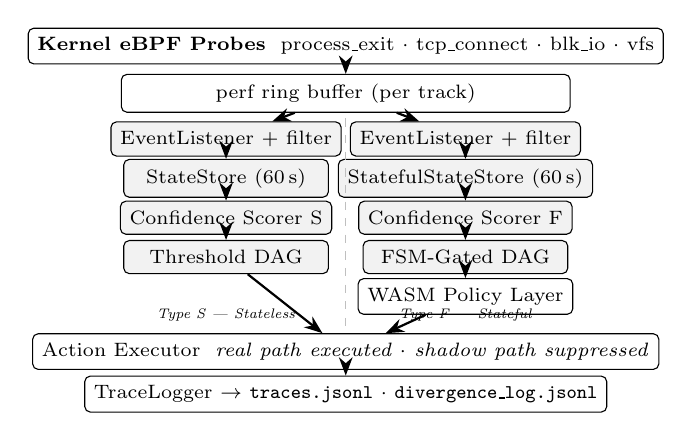
\begin{tikzpicture}[
  font=\scriptsize,
  box/.style={draw, rounded corners=2pt, minimum width=2.6cm,
              minimum height=0.42cm, align=center, fill=white},
  sbox/.style={draw, rounded corners=2pt, minimum width=2.6cm,
               minimum height=0.42cm, align=center, fill=gray!10},
  arr/.style={->,>=Stealth, thick},
  wide/.style={draw, rounded corners=2pt, minimum width=5.7cm,
               minimum height=0.42cm, align=center, fill=white},
]
% ---- Kernel layer ----
\node[wide] (ebpf) at (0, 3.0)
  {\textbf{Kernel eBPF Probes}~~process\_exit $\cdot$ tcp\_connect $\cdot$ blk\_io $\cdot$ vfs};

% ---- perf buffer ----
\node[wide] (buf) at (0, 2.4) {perf ring buffer (per track)};
\draw[arr] (ebpf) -- (buf);

% ---- Two tracks side by side ----
\node[sbox] (esS)  at (-1.52, 1.82) {EventListener~+~filter};
\node[sbox] (esF)  at ( 1.52, 1.82) {EventListener~+~filter};
\node[sbox] (ssS)  at (-1.52, 1.32) {StateStore (60\,s)};
\node[sbox] (ssF)  at ( 1.52, 1.32) {StatefulStateStore (60\,s)};
\node[sbox] (scS)  at (-1.52, 0.82) {Confidence Scorer S};
\node[sbox] (scF)  at ( 1.52, 0.82) {Confidence Scorer F};
\node[sbox] (dagS) at (-1.52, 0.32) {Threshold DAG};
\node[sbox] (dagF) at ( 1.52, 0.32) {FSM-Gated DAG};
\node[box]  (pol)  at ( 1.52,-0.18) {WASM Policy Layer};

% Type labels
\node[font=\tiny\itshape] at (-1.52,-0.42) {Type S --- Stateless};
\node[font=\tiny\itshape] at ( 1.52,-0.42) {Type F --- Stateful};

% Vertical arrows within each track
\foreach \a/\b in {buf/esS, esS/ssS, ssS/scS, scS/dagS}
  \draw[arr] (\a) -- (\b);
\foreach \a/\b in {buf/esF, esF/ssF, ssF/scF, scF/dagF, dagF/pol}
  \draw[arr] (\a) -- (\b);

% ---- Shared action executor ----
\node[wide] (exec) at (0,-0.88)
  {Action Executor~~\textit{real path executed $\cdot$ shadow path suppressed}};
\draw[arr] (dagS) -- (exec);
\draw[arr] (pol)  -- (exec);

% ---- Output ----
\node[wide] (trace) at (0,-1.42)
  {TraceLogger $\rightarrow$ \texttt{traces.jsonl} $\cdot$ \texttt{divergence\_log.jsonl}};
\draw[arr] (exec) -- (trace);

% Vertical divider between tracks
\draw[dashed, gray!50] (0, 2.08) -- (0, -0.55);
\end{tikzpicture}
\caption{Dual-track control plane. Type~S (left) and Type~F (right) share the eBPF bus but run independent scorers and decision engines. Type~F adds an FSM-gated DAG and a WASM policy enforcement layer. Every cycle runs on both a real and shadow path; divergences increment metric~M2.}
\label{fig:arch}
\end{figure}

\section{Type S: Stateless Control Plane}
\label{sec:types}

\subsection{Kernel Probes and Confidence Scoring}

Type~S attaches a tracepoint on \texttt{sched\_process\_exit} and a kprobe on \texttt{tcp\_connect} capturing all connection attempts; elevated connection activity in the window is treated as a proxy for connectivity stress. Per-signal scores for container $c$ and window $W$:

\begin{equation}
s_{\mathrm{pe}}(c, W) = \sigma_{\mathrm{pe}} \cdot \mathbb{1}\!\left[n_{\mathrm{pe}}(c, W) > 0\right]
\label{eq:spe}
\end{equation}

\begin{equation}
s_{\mathrm{tc}}(c, W) = \min\!\left(\frac{n_{\mathrm{tc}}(c, W)}{\theta_{\mathrm{tc}}},\, 1\right) \cdot \sigma_{\mathrm{tc}}
\label{eq:stc}
\end{equation}

Parameters: $\sigma_{\mathrm{pe}} = 0.95$, $\sigma_{\mathrm{tc}} = 0.90$, $\theta_{\mathrm{tc}} = 5$. Scaling TCP activity by count means a single connection attempt will not cross the action threshold. The combined score:

\begin{equation}
\rho_S(c, W) = \max(s_{\mathrm{pe}}(c, W),\, s_{\mathrm{tc}}(c, W))
\label{eq:rhoS}
\end{equation}

\subsection{Decision DAG}

Type~S maps $\rho_S$ to three actions. Thresholds: $\tau_{\mathrm{restart}} = 0.80$, $\tau_{\mathrm{reschedule}} = 0.95$:

\begin{equation*}
\delta_S(c) =
\begin{cases}
\texttt{reschedule} & \text{if } \rho_S \geq \tau_{\mathrm{reschedule}} \\
\texttt{restart}    & \text{if } \tau_{\mathrm{restart}} \leq \rho_S < \tau_{\mathrm{reschedule}} \\
\texttt{no\_action} & \text{if } \rho_S < \tau_{\mathrm{restart}}
\end{cases}
\end{equation*}

Both actions are reversible. No FSM is needed on the Type~S track---stateless workloads carry no on-disk state that an untimely restart can damage.

\section{Type F: Stateful Control Plane}
\label{sec:typef}

\subsection{Kernel Probes and Confidence Scoring}

Type~F attaches kprobes on \texttt{blk\_account\_io\_start/done}, kretprobes on \texttt{vfs\_write/read}, and tracepoints on \texttt{sys\_enter\_umount/mount}. These produce \texttt{blk\_io\_latency}, VFS error, and volume mount events. Let $n_h(c, W)$ be the count of high-latency I/O events (\texttt{latency\_us} $\geq \Lambda = 10{,}000\,\mu$s), $n_{\mathrm{vfs}}(c, W)$ the VFS error count, and $\mathbb{1}_{\mathrm{vol}}(c, W) = 1$ when an unresolved mount loss is present in the window.

\begin{equation}
s_{\mathrm{io}}(c, W) = \min\!\left(\frac{n_h(c, W)}{\theta_{\mathrm{io}}},\, 1\right) \cdot \sigma_{\mathrm{io}}
\label{eq:sio}
\end{equation}

\begin{equation}
s_{\mathrm{vfs}}(c, W) = \min\!\left(\frac{n_{\mathrm{vfs}}(c, W)}{\theta_{\mathrm{vfs}}},\, 1\right) \cdot \sigma_{\mathrm{vfs}}
\label{eq:svfs}
\end{equation}

\begin{equation}
s_{\mathrm{vol}}(c, W) = \sigma_{\mathrm{vol}} \cdot \mathbb{1}_{\mathrm{vol}}(c, W)
\label{eq:svol}
\end{equation}

Parameters: $\theta_{\mathrm{io}} = 5$, $\sigma_{\mathrm{io}} = 0.85$, $\theta_{\mathrm{vfs}} = 3$, $\sigma_{\mathrm{vfs}} = 0.88$, $\sigma_{\mathrm{vol}} = 0.97$. The combined score is:

\begin{equation}
\rho_F(c, W) = \max(s_{\mathrm{io}}(c, W),\, s_{\mathrm{vfs}}(c, W),\, s_{\mathrm{vol}}(c, W))
\label{eq:rhoF}
\end{equation}

\subsection{Five-State FSM}

Table~\ref{tab:fsm} and Fig.~\ref{fig:fsm} give the full transition relation. The FSM persists across cycles and resets only when a complete recovery finishes. The key constraint is Degraded$\rightarrow$Audited: \texttt{checkpoint\_and\_restart} (implemented using CRIU~\cite{b2}) cannot fire in the same reconcile cycle as the first fault-triggered \texttt{flush\_io\_queue}. Algorithm~\ref{alg:reconcile} shows why: the audit transition (step~4b) fires in the same call that downgrades C\&R to flush (step~4a), so C\&R can only execute in the following cycle at earliest. At minimum one reconcile interval (5\,s) separates first fault detection from checkpoint execution.

\begin{table}[!t]
\caption{TYPE F FSM TRANSITION RELATION.}
\label{tab:fsm}
\centering
\renewcommand{\arraystretch}{1.15}
\resizebox{\columnwidth}{!}{%
\begin{tabular}{llll}
\hline
\textbf{From} & \textbf{Trigger} & \textbf{To} & \textbf{Condition} \\
\hline
Healthy   & \texttt{degrade}         & Degraded  & $\rho_F \geq \tau_{\mathrm{flush}}$ \\
Degraded  & \texttt{audit}           & Audited   & \texttt{flush\_io\_queue} executed \\
Degraded  & \texttt{degrade}         & Degraded  & score re-confirmed; state held \\
Audited   & \texttt{approve\_repair} & Repairing & \texttt{checkpoint\_and\_restart} approved \\
Audited   & \texttt{degrade}         & Degraded  & fault worsens during audit phase \\
Repairing & \texttt{recover}         & Recovered & action succeeded \\
Repairing & \texttt{degrade}         & Degraded  & repair fails; restart fault path \\
Recovered & \texttt{heal}            & Healthy   & $\rho_F < \tau_{\mathrm{flush}}$ \\
Recovered & \texttt{degrade}         & Degraded  & $\rho_F \geq \tau_{\mathrm{flush}}$ (re-fault) \\
\hline
\end{tabular}%
}
\end{table}

\begin{figure}[!t]
\centering
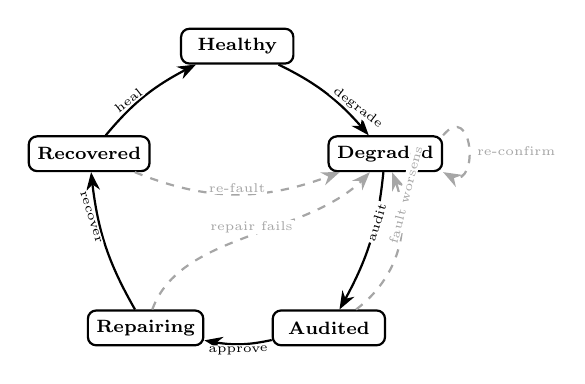
\begin{tikzpicture}[
  ->, >=Stealth, thick,
  st/.style={draw, rounded corners=3pt,
             minimum width=1.55cm, minimum height=0.48cm,
             align=center, font=\scriptsize\bfseries, fill=white},
  lbl/.style={font=\tiny, fill=white, inner sep=0.5pt, sloped},
  scale=0.92, transform shape,
]
% Pentagon layout: radius=2.15, clockwise from 90 deg
% Angles: Healthy=90, Degraded=18, Audited=306, Repairing=234, Recovered=162
\node[st] (H) at ( 0.000,  2.150) {Healthy};
\node[st] (D) at ( 2.044,  0.665) {Degraded};
\node[st] (A) at ( 1.265, -1.739) {Audited};
\node[st] (R) at (-1.265, -1.739) {Repairing};
\node[st] (V) at (-2.044,  0.665) {Recovered};

% --- Forward arcs (clockwise, solid) ---
\draw (H) to[bend left=12]  node[lbl, above right]{degrade}    (D);
\draw (D) to[bend left=12]  node[lbl, right]      {audit}      (A);
\draw (A) to[bend left=12]  node[lbl, below]      {approve}    (R);
\draw (R) to[bend left=12]  node[lbl, below left] {recover}    (V);
\draw (V) to[bend left=12]  node[lbl, above left] {heal}       (H);

% --- Back-edges (dashed, gray) ---
% Self-loop on Degraded (exit NE, return SE)
\draw[dashed,gray!70] (D.north east)
    to[out=50, in=320, looseness=3.5]
    node[lbl, right=2pt, sloped=false]{\tiny re-confirm}
    (D.south east);
% Audited -> Degraded (fault worsens)
\draw[dashed,gray!70] (A) to[bend right=38]
    node[lbl, above right]{\tiny fault worsens} (D);
% Repairing -> Degraded (repair fails)
\draw[dashed,gray!70] (R) to[out=70, in=230, looseness=0.85]
    node[lbl, above, sloped=false]{\tiny repair fails} (D);
% Recovered -> Degraded (re-fault)
\draw[dashed,gray!70] (V) to[bend right=22]
    node[lbl, above]{\tiny re-fault} (D);
\end{tikzpicture}
\caption{Type~F five-state FSM. Solid clockwise arcs follow the nominal recovery path. Dashed arcs route recurrences and failures back to Degraded. \texttt{checkpoint\_and\_restart} is only reachable from Audited, enforcing at least one 5\,s reconcile interval between first fault detection and checkpoint dispatch.}
\label{fig:fsm}
\end{figure}

\subsection{FSM-Gated Reconciliation and Policy Layer}

\begin{algorithm}
\caption{Type~F FSM-Gated Reconciliation (single container $c$)}
\label{alg:reconcile}
\begin{algorithmic}[1]
\REQUIRE StateStore $\mathcal{S}$, FSM $\mathcal{F}$, container $c$
\ENSURE Decision record with \textit{action} and \textit{blocked\_reason}
\STATE $\rho \leftarrow \rho_F(c, \mathcal{S})$;\ $\mathit{sig} \leftarrow \mathrm{KernelSignals}(\mathcal{S}, c)$;\ $q \leftarrow \mathcal{F}.\mathrm{state}(c)$
\STATE \textit{--- (1) Raw DAG ---}
\IF{$\rho \geq \tau_{\mathrm{escalate}}$}
    \STATE $\mathit{raw} \leftarrow \texttt{escalate}$
\ELSIF{$\rho \geq \tau_{\mathrm{repair}}$}
    \STATE $\mathit{raw} \leftarrow \texttt{C\&R}$
\ELSIF{$\rho \geq \tau_{\mathrm{flush}}$}
    \STATE $\mathit{raw} \leftarrow \texttt{flush}$
\ELSE
    \STATE $\mathit{raw} \leftarrow \texttt{no\_action}$
\ENDIF
\STATE $\mathit{act} \leftarrow \mathit{raw}$
\STATE \textit{--- (2) Reversibility gate ---}
\IF{$\mathit{raw} \in \mathit{IrreversibleActions}$}
    \STATE $\mathit{act} \leftarrow \texttt{no\_action}$; set \textit{blocked\_reason}
\ENDIF
\STATE \textit{--- (3) FSM degrade ---}
\IF{$\rho \geq \tau_{\mathrm{flush}}$ \AND $\mathit{act} \neq \texttt{no\_action}$ \AND $q \in \{\textit{Healthy}, \textit{Recovered}\}$}
    \STATE $\mathcal{F}.\mathrm{apply}(c, \texttt{degrade})$;\ $q \leftarrow \mathcal{F}.\mathrm{state}(c)$
\ENDIF
\STATE \textit{--- (4) FSM gates ---}
\IF{$\mathit{act} = \texttt{C\&R}$ \AND $q \neq \textit{Audited}$}
    \STATE $\mathit{act} \leftarrow \texttt{flush}$; set \textit{blocked\_reason} \COMMENT{must audit before repair}
\ENDIF
\IF{$\mathit{act} = \texttt{flush}$ \AND $q = \textit{Degraded}$}
    \STATE $\mathcal{F}.\mathrm{apply}(c, \texttt{audit})$;\ $q \leftarrow \mathcal{F}.\mathrm{state}(c)$ \COMMENT{Degraded $\rightarrow$ Audited}
\ENDIF
\IF{$\mathit{act} = \texttt{C\&R}$ \AND $q = \textit{Audited}$}
    \STATE $\mathcal{F}.\mathrm{apply}(c, \texttt{approve\_repair})$ \COMMENT{Audited $\rightarrow$ Repairing}
\ENDIF
\IF{$\mathit{act} = \texttt{escalate}$ \AND $q \notin \{\textit{Degraded}, \textit{Audited}, \textit{Repairing}\}$}
    \STATE $\mathit{act} \leftarrow \texttt{flush}$; set \textit{blocked\_reason} \COMMENT{escalate gate}
\ENDIF
\STATE \textit{--- (5) Heal ---}
\IF{$\rho < \tau_{\mathrm{flush}}$ \AND $q = \textit{Recovered}$}
    \STATE $\mathcal{F}.\mathrm{apply}(c, \texttt{heal})$ \COMMENT{Recovered $\rightarrow$ Healthy}
\ENDIF
\RETURN $(c,\, \rho,\, \mathit{act},\, \mathit{sig},\, \mathcal{F}.\mathrm{state}(c),\, \mathit{blocked\_reason})$
\end{algorithmic}
\end{algorithm}

Thresholds: $\tau_{\mathrm{flush}} = 0.50$, $\tau_{\mathrm{repair}} = 0.80$, $\tau_{\mathrm{escalate}} = 0.95$. \texttt{C\&R} abbreviates \texttt{checkpoint\_and\_restart}; \texttt{flush} abbreviates \texttt{flush\_io\_queue}; $q = \mathcal{F}.\mathrm{state}(c)$.

Algorithm~\ref{alg:reconcile} gives the full reconcile procedure. On the real path the FSM is mutated in-place; on the shadow path a fresh copy runs and is then discarded. Between the DAG output and the action executor sits a pluggable policy layer that re-checks FSM sequence constraints as an independent second enforcement point~\cite{b4}. The WASM sandbox is validated separately (§\ref{sec:limitations}); the fault-injection campaign and trace corpus predate wasmtime activation, so M6 counts Python-gate suppressions only (Table~\ref{tab:metrics}, footnote~$^{b}$).

\section{Research Metrics and Evaluation Framework}
\label{sec:metrics}

Six metrics are defined over $\mathcal{T}$ (all traces), with $\mathcal{T}_{\mathrm{real}}$ denoting the real-path subset and $\mathcal{T}_{\mathrm{active}} = \{t \in \mathcal{T}_{\mathrm{real}} : \mathrm{action}(t) \neq \texttt{no\_action}\}$. M1 and M5 are schema validation checks that verify trace correctness; M2, M3, M4, and M6 are the behavioural research metrics.

\textbf{M1: Cross-Track Contamination Check.} The fraction of records carrying signals inconsistent with their \texttt{node\_type} label.
\begin{equation}
M_1 = \frac{|\{t \in \mathcal{T} : \mathrm{misclassified}(t)\}|}{|\mathcal{T}|}
\label{eq:M1}
\end{equation}

\textbf{M2: Divergence Rate.} The fraction of real-path cycles where the real and shadow actions disagree.
\begin{equation}
M_2 = \frac{|\{t \in \mathcal{T}_{\mathrm{real}} : a_{\mathrm{real}}(t) \neq a_{\mathrm{shadow}}(t)\}|}{|\mathcal{T}_{\mathrm{real}}|}
\label{eq:M2}
\end{equation}

\textbf{M3: Mean Time To Recovery.} Mean wall-clock duration from fault injection to first \texttt{checkpoint\_and\_restart} dispatch, measured per-episode by \texttt{scripts/run\_episodes.py}.
\begin{equation}
M_3 = \frac{1}{|\mathcal{E}|} \sum_{e \in \mathcal{E}} \!\left(t_{\mathrm{cr}}(e) - t_{\mathrm{fault}}(e)\right)
\label{eq:M3}
\end{equation}

\textbf{M4: Reversibility Ratio.}
\begin{equation}
M_4 = \frac{|\{t \in \mathcal{T}_{\mathrm{active}} : \mathrm{reversible}(t)\}|}{|\mathcal{T}_{\mathrm{active}}|}
\label{eq:M4}
\end{equation}

\textbf{M5: Explanation Field Completeness Check.} The fraction of records where all required fields are non-empty: \texttt{why}, \texttt{action}, \texttt{score}, \texttt{kernel\_signals} (may be empty for \texttt{no\_action} decisions), and \texttt{dag\_pattern}.
\begin{equation}
M_5 = \frac{|\{t \in \mathcal{T} : \mathrm{complete}(t)\}|}{|\mathcal{T}|}
\label{eq:M5}
\end{equation}

\textbf{M6: Unsafe-Action Suppression Rate.} The fraction of real-path records where the FSM gate or policy layer overrode the raw DAG action.
\begin{equation}
M_6 = \frac{|\{t \in \mathcal{T}_{\mathrm{real}} : \mathrm{suppressed}(t)\}|}{|\mathcal{T}_{\mathrm{real}}|}
\label{eq:M6}
\end{equation}

\subsection{Cross-Controller Scenario Table}

\begin{table*}[!t]
\caption{CROSS-CONTROLLER FUNCTIONAL CORRECTNESS SCENARIOS. ALL SCENARIOS PASSED.}
\label{tab:scenarios}
\centering
\renewcommand{\arraystretch}{1.15}
\begin{tabular}{llcll}
\hline
\textbf{Track} & \textbf{Scenario} & \textbf{Score} & \textbf{Expected} & \textbf{Observed} \\
\hline
S & Sub-threshold     & 0.54                  & \texttt{no\_action}           & \texttt{no\_action} \\
S & Minor fault       & 0.90                  & \texttt{restart}              & \texttt{restart} \\
S & Critical fault    & 0.95                  & \texttt{reschedule}           & \texttt{reschedule} \\
S & Recovery          & 0.95$\rightarrow$drop & \texttt{reschedule}           & \texttt{reschedule} \\
F & Sub-threshold     & 0.29                  & \texttt{no\_action}           & \texttt{no\_action} \\
F & Minor (flush)     & 0.59                  & \texttt{flush\_io\_queue}     & \texttt{flush\_io\_queue} \\
F & Major (FSM-gated) & 0.85                  & \texttt{flush\_io\_queue}$^{a}$ & \texttt{flush\_io\_queue} \\
F & Critical          & 0.97                  & \texttt{escalate}             & \texttt{escalate} \\
F & Recovery          & 0.59$\rightarrow$drop & \texttt{flush\_io\_queue}     & \texttt{flush\_io\_queue} \\
\hline
\multicolumn{5}{l}{\footnotesize $^{a}$FSM in Degraded (not Audited); \texttt{checkpoint\_and\_restart} deferred to \texttt{flush\_io\_queue}.}
\end{tabular}
\end{table*}

\section{Evaluation}
\label{sec:eval}

The evaluation addresses four questions. (1)~Does FSM history change decisions in practice compared to a memoryless baseline? (2)~How long does recovery take under controlled fault injection, and how consistently? (3)~Are all dispatched actions reversible? (4)~What does the FSM contribute, and what happens without it? M1, M2, M4--M6 derive from the committed \texttt{data/phase2/} trace snapshot. M3 uses a synthetic fault-injection harness (§\ref{sec:m3}).

\subsection{Experimental Setup}

The host was an x86-64 workstation running Ubuntu~22.04 (Linux~5.15), with 8\,GB RAM and a 64\,GB HDD-backed virtual disk. eBPF attachment used BCC and required root. Four Docker containers ran as monitored targets: \texttt{nginx} (Type~S track), \texttt{postgres} (with a persistent volume), \texttt{redis}, and \texttt{mysql} (Type~F track). All four appear in the committed trace corpus. Episode data for \texttt{postgres} and \texttt{mysql} MTTR runs was not committed (see §\ref{sec:limitations}). Reconcile interval was 5\,s; sliding event window was 60\,s. Decisions logged to \texttt{traces.jsonl} (schema version~1.3.0). No external Docker operations were performed independently of the remediation controller during evaluation; all container interactions were dispatched by the action executor as recorded in the trace logs.

The committed evaluation snapshot (\texttt{data/phase2/}) contains 9,132 total traces: 4,564 stateful (2,282 real, 2,282 shadow) and 4,568 stateless (2,284 real, 2,284 shadow). Of 2,282 real stateful cycles, 2,187 (95.8\,\%) produced \texttt{no\_action} and 95 (4.2\,\%) were active interventions (51 \texttt{flush\_io\_queue}, 44 \texttt{checkpoint\_and\_restart}). The high \texttt{no\_action} fraction confirms the controller does not fire spuriously: during cycles where the score is below $\tau_{\mathrm{flush}} = 0.50$, both the real FSM and the shadow FSM agree, and M2 is unaffected. The 44 divergences arise exclusively in cycles where the real FSM, having accumulated Audited state, approves \texttt{checkpoint\_and\_restart} while the fresh-each-cycle shadow FSM can only reach Degraded and defers to \texttt{flush\_io\_queue}.

\subsection{Trace-Based Metric Results}

$M_1 = 0.0000$; $M_5 = 1.0000$ (schema validation checks). Across 9,132 total traces (2,282 + 2,284 real; 2,282 + 2,284 shadow), no record carried signals inconsistent with its \texttt{node\_type} label, and every record had all required explanation fields populated. For \texttt{no\_action} decisions, \texttt{kernel\_signals} may be empty by design (no fault signal is present); the completeness check accepts this as valid. These confirm schema correctness across the full committed corpus.

$M_4 = 1.0000$. All 95 active Type-F decisions were reversible: 51 \texttt{flush\_io\_queue} and 44 \texttt{checkpoint\_and\_restart}, both tagged \texttt{reversibility="reversible"} in the trace schema. The \texttt{volume\_delete} action (irreversible) and \texttt{escalate} action (\texttt{reversibility="conditional"} in the schema) were never triggered by the observed fault patterns. M4\,=\,1.0000 therefore confirms that the reversibility gate never needed to activate during this evaluation; had \texttt{escalate} fired, its ``conditional'' tag would exclude it from the numerator and reduce M4 below 1.0.

$M_2 = M_6 = 0.0193$ (Type-F track, 44 of 2,282 real stateful cycles). In every case the divergence pattern was the same: the real FSM had accumulated enough state to reach Audited and approve \texttt{checkpoint\_and\_restart}; the shadow FSM, reset each cycle, only reached Degraded and deferred to \texttt{flush\_io\_queue}. All 44 divergence records appear in \texttt{stateful\_divergence\_log.jsonl} with the pair \texttt{checkpoint\_and\_restart}$\rightarrow$\texttt{flush\_io\_queue}. The stateless track produces zero divergences by construction: the Type~S shadow path runs the same stateless threshold DAG as the real path and cannot accumulate state that would cause disagreement. Hence $M_2^\mathrm{S} = 0.0000$ and the per-track values are $M_2^\mathrm{F} = 0.0193$, $M_2^\mathrm{overall} = 0.0096$.

The equality $M_2 = M_6 = 0.0193$ is a structural consequence of the episode lifecycle, not a definitional equivalence. The two metrics count \emph{different} cycle instances within the same 44 fault episodes. Each episode contributes one M6 cycle (cycle~1: the real FSM, in Degraded, blocks C\&R on the real path and records \texttt{flush} with \texttt{blocked\_reason} set; the shadow FSM is also in Degraded and also produces \texttt{flush}---no divergence occurs) and one M2 cycle (cycle~2: the real FSM, now in Audited, approves C\&R while the fresh-each-cycle shadow FSM, still in Degraded, defers to \texttt{flush}---a logged divergence). The M6 cycles are not divergent; the M2 cycles are not suppressed. The count coincides at 44 because each of the 44 recovered fault episodes contributes exactly one of each type.

\subsection{Fault-Injection MTTR Campaign}
\label{sec:m3}

$M_3$ was measured by the \texttt{scripts/run\_episodes.py} harness. Each episode: inject eight \texttt{blk\_io\_latency} events (50--54\,ms, above the $\Lambda = 10{,}000\,\mu$s threshold) directly into a fresh \texttt{StatefulStateStore}; reconcile every 5\,s until \texttt{checkpoint\_and\_restart} fires or 60\,s elapses; record wall time from injection to first C\&R dispatch (MTTR). This definition captures the structural FSM two-cycle delay: \texttt{flush\_io\_queue} fires in cycle~1 (FSM: Healthy$\rightarrow$Degraded$\rightarrow$Audited), and \texttt{checkpoint\_and\_restart} is approved in cycle~2.

Episode data is committed for \texttt{redis} only ($N = 30$, \texttt{scripts/mttr\_summary.json}): mean MTTR $10.40$\,s, $\sigma = 0.03$\,s, min $10.34$\,s, max $10.50$\,s, $\sigma/\mu = 0.25\%$ (Fig.~\ref{fig:mttr}). Every episode followed the identical two-cycle action sequence. Episode files for \texttt{postgres} and \texttt{mysql} were not committed and their MTTR values are not available from the current repository state (see §\ref{sec:limitations}).

\begin{figure}[!t]
\centering
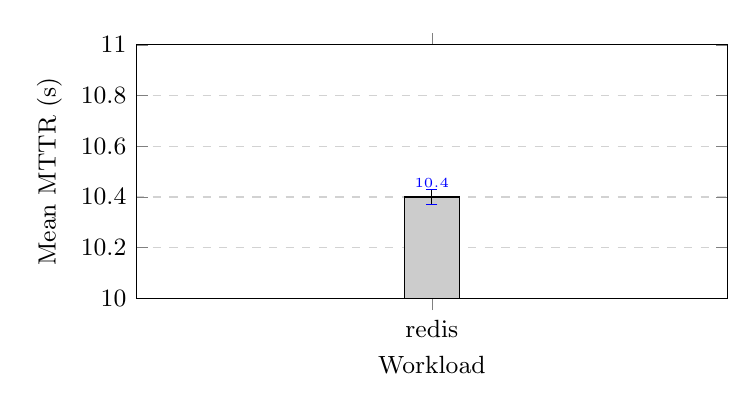
\begin{tikzpicture}
\begin{axis}[
  ybar,
  bar width=0.70cm,
  xlabel={Workload},
  ylabel={Mean MTTR (s)},
  xlabel style={font=\small},
  ylabel style={font=\small},
  ymin=10.0, ymax=11.0,
  symbolic x coords={redis},
  xtick=data,
  xticklabel style={font=\small},
  yticklabel style={font=\small},
  ytick={10.0,10.2,10.4,10.6,10.8,11.0},
  ymajorgrids=true, grid style={dashed,gray!35},
  enlarge x limits=0.6,
  width=0.75\columnwidth, height=4.8cm,
  every node near coord/.append style={font=\tiny, /pgf/number format/fixed,
    /pgf/number format/precision=2},
  nodes near coords,
  nodes near coords align={above},
]
\addplot+[
  fill=gray!40, draw=black,
  error bars/.cd, y dir=both, y explicit,
] coordinates {
  (redis, 10.40) +- (0, 0.03)
};
\end{axis}
\end{tikzpicture}
\caption{Mean MTTR for \texttt{redis}, $N = 30$ episodes (all recovered). Error bars show $\pm 1\sigma$. $\sigma/\mu = 0.25\%$; the near-zero variance is structural: every episode follows the identical two-cycle FSM sequence. MTTR variation reflects scheduling jitter in the two 5\,s reconcile-interval sleeps (the harness measures time to C\&R decision dispatch; no \texttt{docker restart} is executed during MTTR measurement). Episode data for \texttt{postgres} and \texttt{mysql} was not committed and is not available.}
\label{fig:mttr}
\end{figure}

\begin{table*}[!t]
\caption{METRIC VALUES. M1--M2, M4--M6: DERIVED FROM THE COMMITTED \texttt{data/phase2/} SNAPSHOT ($N = 9{,}132$ TOTAL TRACES; $N_{\mathrm{real}}^{\mathrm{F}} = 2{,}282$, $N_{\mathrm{real}}^{\mathrm{S}} = 2{,}284$). M3: SYNTHETIC FAULT INJECTION HARNESS (\texttt{redis}, $N = 30$ EPISODES).}
\label{tab:metrics}
\centering
\renewcommand{\arraystretch}{1.15}
\begin{tabular}{lcccp{5.5cm}}
\hline
\textbf{Metric} & \textbf{Type S} & \textbf{Type F} & \textbf{Overall} & \textbf{Note} \\
\hline
M1 (misclassification)  & 0.0000 & 0.0000 & 0.0000 & $N = 9{,}132$ traces; zero contaminated records \\
M2 (divergence rate)    & 0.0000 & 0.0193 & 0.0096 & 44 of 2{,}282 real Type-F cycles; 44/4{,}566 overall \\
M3 (MTTR, seconds)      & ---    & 10.40  & ---    & \texttt{redis} only, $N=30$, $\sigma=0.03$\,s ($^{a}$) \\
M4 (reversibility)      & 1.0000 & 1.0000 & 1.0000 & 95 active Type-F decisions (flush=51, C\&R=44) \\
M5 (expl.\ complete)    & 1.0000 & 1.0000 & 1.0000 & Zero missing required fields across 9{,}132 traces \\
M6 (suppression rate)   & 0.0000 & 0.0193 & 0.0096 & 44 FSM-gated actions ($^{b}$) \\
\hline
\multicolumn{5}{l}{\footnotesize $^{a}$All 30 episodes recovered (0 timeouts). Two-cycle sequence confirmed: \texttt{flush\_io\_queue} cycle~1, C\&R cycle~2. Episode data for \texttt{postgres} and \texttt{mysql} not committed.}\\
\multicolumn{5}{l}{\footnotesize $^{b}$Python FSM gate is primary enforcer; this count predates wasmtime activation. WASM sandbox validated separately (all 20 policy cases correct); steady-state overhead 27\,$\mu$s mean, 50\,$\mu$s at p99 ($N = 10{,}000$, §\ref{sec:overhead}).}
\end{tabular}
\end{table*}

\subsection{Cross-Controller Functional Correctness}

All nine scenarios in Table~\ref{tab:scenarios} produced the expected action (accuracy: 1.00). A trial-based functional evaluation across twelve fault scenario types (4 stateful, 8 stateless; $N = 30$ trials each; \texttt{evaluation/results/summary\_table.csv}) confirms this: stateful scenarios (cascade I/O+volume, I/O degradation, VFS errors, volume lost) achieve F1\,=\,1.000 each; stateless scenarios achieve F1\,=\,1.000 for 6 of 8 types (mean decision latency 18.65\,$\mu$s stateful, 11.58\,$\mu$s stateless per \texttt{evaluation/results/latency\_report.csv}). The two undetectable scenarios---\texttt{cpu\_flicker} and \texttt{ambiguous}---yield F1\,=\,0.000 for both the UnderCurrent controller and the naive baseline, confirming these are representational gaps in the signal classes, not controller failures.

\subsection{Baseline Comparison and Ablation}
\label{sec:ablation}

To answer ``why is the FSM necessary?'', we replayed the $N = 2{,}282$ real stateful trace entries from the committed snapshot under three counterfactual decision policies, holding the recorded \texttt{score} values constant while varying only the decision mechanism (Table~\ref{tab:ablation}).

\begin{table}[t]
\caption{Decision-policy ablation on $N = 2{,}282$ real Type-F traces (\texttt{stateful/ablation\_results.json}). Input confidence scores are held constant; only the decision mechanism varies. \emph{Unsafe C\&R}: dispatched from a pre-audit FSM state. \emph{Missed C\&R}: legitimate checkpoint opportunity suppressed by a memoryless or binary policy.}
\label{tab:ablation}
\centering
\begin{tabular}{lrcc}
\hline
Controller & C\&R dispatched & Unsafe C\&R & Missed C\&R \\
\hline
UnderCurrent (full FSM) & 44\;(1.93\%) & 0 & 0 \\
No-FSM (always-restart) & 88\;(3.86\%) & 44 & 0 \\
Threshold-only (shadow) & 0\;\;\;(0\%) & 0 & 44 \\
No-confidence (binary)  & 0\;\;\;(0\%) & 0 & 44$^{c}$ \\
\hline
\multicolumn{4}{p{0.88\columnwidth}}{\footnotesize $^{c}$7 extra \texttt{flush} dispatches (binary score $0.75\geq\tau_{\mathrm{flush}}$) also disagree with baseline \texttt{no\_action}; total disagreements\,=\,51 (\texttt{ablation\_results.json}).} \\
\end{tabular}
\end{table}

\textbf{No-FSM.} Removing FSM state gating doubles the C\&R rate to 88 dispatches; 44 of these are premature---they fire from a pre-audit FSM state where the full controller issues \texttt{flush\_io\_queue} and defers C\&R to the following cycle. All 44 premature dispatches coincide exactly with cycles where the FSM has not yet reached Audited.

\textbf{Threshold-only (shadow path).} A stateless threshold policy---equivalent to instantiating a fresh FSM every cycle---can never reach Audited within a single cycle and therefore never approves C\&R. This variant misses all 44 legitimate C\&R opportunities. Notably, this is the same computation already performed by \texttt{reconcile\_both()} in every cycle: $M_2 = 0.0193$ (44 divergent cycles of 2,282 real stateful cycles) quantifies exactly how often the shadow path would have made the wrong call across the full corpus.

\textbf{No-confidence.} Replacing the continuous score with a binary fault/no-fault signal (score $\in \{0, 0.75\}$) also yields 0 C\&R dispatches, because $0.75 < \tau_{\mathrm{repair}} = 0.80$: every fault cycle is downgraded to \texttt{flush\_io\_queue}. Graduated confidence scoring is necessary for C\&R to be reachable at all.

UnderCurrent dispatches exactly 44 C\&Rs, all from Audited state---zero premature, zero missed. The two alternatives fail in opposite directions: without FSM memory, the controller is too aggressive (fires C\&R before the audit gate); without state accumulation, it is too conservative (never fires C\&R). The FSM threads the needle by accumulating evidence across cycles before approving the irreversible action.

\subsection{Threshold Sensitivity}
\label{sec:sensitivity}

Three hyperparameters were swept independently, holding all others at nominal values. For each setting, the controller was evaluated over its full fault scenario set. Table~\ref{tab:sensitivity} reports macro-averaged F1 across scenarios (\texttt{evaluation/results/sensitivity\_results.csv}).

\begin{table}[t]
\caption{THRESHOLD SENSITIVITY (MACRO-AVERAGED F1 OVER FAULT SCENARIOS; EACH PARAMETER SWEPT INDEPENDENTLY; \texttt{evaluation/results/sensitivity\_results.csv}).}
\label{tab:sensitivity}
\centering
\renewcommand{\arraystretch}{1.15}
\begin{tabular}{lrl}
\hline
\textbf{Parameter} & \textbf{Values tested} & \textbf{Mean F1} \\
\hline
FLUSH\_THRESHOLD (Type F) & 0.30--0.70 & 1.000, constant \\
\texttt{window\_seconds} (both)    & 15--240\,s & 0.833, constant \\
$\tau_{\mathrm{restart}}$ (Type S) & 0.60--0.90 & 0.750, constant \\
$\tau_{\mathrm{restart}}$ (Type S) & 0.95       & 0.375 \\
\hline
\end{tabular}
\end{table}

\textbf{FLUSH\_THRESHOLD} is the most stable parameter: F1\,=\,1.000 across the entire 0.30--0.70 range. The result follows from the FSM structure. The flush threshold controls when a container first enters Degraded; the FSM then requires a Degraded$\rightarrow$Audited transition on the subsequent cycle before any \texttt{checkpoint\_and\_restart} is approved. That sequencing constraint is enforced by the algorithm, not by the threshold value---so long as $\tau_{\mathrm{flush}}$ is low enough to detect real faults, decision quality is unaffected by its exact value.

\textbf{window\_seconds} is equally stable: F1\,=\,0.833 from 15\,s to 240\,s. Two fault scenarios (\texttt{cpu\_flicker}, \texttt{ambiguous}) are inherently not representable by either scorer's signal classes and remain undetectable at any window length; all other scenarios are consistently detected. The count-based scoring model accumulates evidence proportionally to window size, making it insensitive to window length above the minimum needed to observe a single event.

\textbf{$\tau_{\mathrm{restart}}$} holds at F1\,=\,0.750 for 0.60--0.90, then falls to 0.375 at $\tau_{\mathrm{restart}} = 0.95$. The drop occurs because at this value $\tau_{\mathrm{restart}} = \tau_{\mathrm{reschedule}}$, collapsing the restart band: scores in [0.80, 0.94] that would normally dispatch \texttt{restart} instead produce \texttt{no\_action}. The nominal value 0.80 provides 0.15 margin below the reschedule threshold, making this boundary condition avoidable by construction.

\subsection{Runtime Overhead}
\label{sec:overhead}

Two sources of per-cycle overhead are evaluated (Table~\ref{tab:overhead}; \texttt{results/overhead\_benchmark.json}, $N = 10{,}000$ post-warmup calls).

\begin{table}[t]
\caption{Runtime overhead (WASM: $N = 10{,}000$ calls post JIT warmup; shadow: $N = 2{,}000$ calls; \texttt{results/overhead\_benchmark.json}). Both costs are negligible relative to the 5\,s reconcile interval.}
\label{tab:overhead}
\centering
\begin{tabular}{lrrrr}
\hline
Component & Mean & p95 & p99 & Interval\,\% \\
\hline
WASM \texttt{policy\_check()} & 27\,$\mu$s & 30\,$\mu$s & 50\,$\mu$s & 0.0005\,\% \\
Shadow execution (overhead) & 8\,$\mu$s & --- & --- & 0.0002\,\% \\
\hline
\end{tabular}
\end{table}

\textbf{WASM policy sandbox.} Each \texttt{policy\_check()} call creates a fresh \texttt{Store} and \texttt{Instance} from a pre-compiled cached module; compilation is amortised at process startup. Across 10{,}000 post-warmup calls (2{,}500 per action module) the mean is 27.19\,$\mu$s (stddev 12.30\,$\mu$s, p95 29.58\,$\mu$s, p99 50.42\,$\mu$s). An equivalent pure-Python FSM state lookup costs 0.12\,$\mu$s (mean; p50: 0.125\,$\mu$s); the sandbox adds $230{\times}$ the raw decision cost. In absolute terms 27\,$\mu$s is 0.0005\,\% of the 5\,s reconcile interval, making the overhead inconsequential for the target operating cadence.

\textbf{Shadow execution.} Running \texttt{reconcile\_both()} (real FSM + throwaway shadow FSM) takes 14.94\,$\mu$s versus 6.89\,$\mu$s for a single \texttt{reconcile()} call---an 8.06\,$\mu$s absolute overhead, 117\,\% of single-path cost. The proportional figure is large because both paths perform equivalent decision work; the absolute cost is negligible because the control loop sleeps 5\,s between iterations. This confirms that shadow execution is a practical instrument for production deployment, not a research-only technique.

\section{Discussion}
\label{sec:discussion}

\subsection{Design Choices}

\textbf{Scoring model.} The max combiner in~\eqref{eq:rhoS} and~\eqref{eq:rhoF} ensures that a quiescent signal class cannot suppress the dominant fault indicator: a container with frequent process exits but no TCP failures scores at $\sigma_{\mathrm{pe}} = 0.95$, independent of $s_{\mathrm{tc}}$. Score ceilings below 1.0 deliberately leave the top of $[0, 1]$ open for future signal classes with higher diagnostic confidence---hardware error counters, OOM events, or CPU throttling events---without requiring threshold re-calibration across existing signals. The sensitivity analysis (§\ref{sec:sensitivity}) confirms that the exact threshold values are not critical within the tested range.

\textbf{Type~S has no FSM} because stateless workloads carry no on-disk state that an untimely restart can corrupt; audit-phase sequencing would add one full reconcile interval of latency with no corresponding safety benefit. Shadow computation on the Type~S track is therefore always identical to the real path---real and shadow actions agree on every cycle by construction---so M2 is informative only on the Type~F track, where accumulated FSM state causes the paths to diverge.

\textbf{Divergence rate interpretation.} $M_2^\mathrm{F} = 0.0193$ means FSM history changes the dispatched action in 1.93\% of all real stateful cycles. This is not a measure of how often \texttt{checkpoint\_and\_restart} is appropriate; it is a measure of how often the presence of accumulated state changes what is dispatched. The 44 divergent cycles account for all 44 committed C\&R dispatches: every C\&R in the trace corpus required FSM memory to authorise it, and every FSM-memory-dependent decision in the corpus was a C\&R.

\subsection{Limitations}
\label{sec:limitations}

\textbf{Platform scope.} Experiments ran on a developer workstation running Linux~5.15, not a Kubernetes cluster. The eBPF probe architecture requires Linux~4.9+; specific kprobe attachment points may need updating on kernels that have renamed the relevant symbols. Workload classification is static at configuration time; runtime reclassification is not supported.

\textbf{CRIU and checkpoint restore.} CRIU checkpoint creation (\texttt{docker checkpoint create}) was exercised on \texttt{redis} during development and observed to produce a checkpoint artefact with exit code~0; no committed test log corroborates this observation. Restore via \texttt{docker start --checkpoint} fails on this host due to a network-namespace bind-mount limitation in Linux~5.15; the restored process cannot re-attach to its original netns, so recovery falls back to \texttt{docker restart}. The FSM sequencing guarantee---that \texttt{checkpoint\_and\_restart} cannot fire before the audit phase completes---is fully exercised at the decision layer; the checkpoint artefact is created; only the in-place memory restore is constrained by the kernel. Quantitative CRIU checkpoint-creation latency measurements for \texttt{postgres} and \texttt{mysql} were not committed to the repository and are not available from the current codebase.

\textbf{Fault injection and workload coverage.} $M_3$ is based on $N = 30$ synthetic fault episodes on \texttt{redis} (all recovered). MTTR data for \texttt{postgres} and \texttt{mysql} was not committed and cannot be reported. Fault injection inserts \texttt{blk\_io\_latency} events directly into a fresh \texttt{StatefulStateStore}, bypassing eBPF; real VFS fault injection via \texttt{/dev/full} or \texttt{stress-ng} would connect detection and recovery into a single observable latency. The two undetectable fault scenarios (\texttt{cpu\_flicker}, \texttt{ambiguous}) indicate a representational gap: neither scorer's signal classes capture CPU-frequency transients or ambiguous co-occurrence patterns.

\textbf{WASM policy sandbox.} The sandbox (\texttt{wasmtime}~45.0.0) is validated: all four action modules compile and execute, \texttt{policy\_check()} returns the correct verdict in all 20 test cases, and steady-state overhead is 27\,$\mu$s mean (50\,$\mu$s at p99, $N = 10{,}000$ post-warmup). The trace corpus and ablation study predate wasmtime activation; M6 counts therefore reflect Python-gate suppressions only.

\subsection{Future Work}

Deploying on a real Kubernetes cluster is the obvious next step---the per-host eBPF model would be replaced by a DaemonSet-based probe agent, enabling evaluation across multi-node workloads. CRIU restore via \texttt{docker start --checkpoint} currently fails on Linux~5.15 due to a netns bind-mount limitation; testing on a newer kernel or with rootful containers is a concrete near-term step. Committing per-workload episode files for \texttt{postgres} and \texttt{mysql} would complete the M3 MTTR picture across the three stateful targets. A fault-injection harness using real VFS errors (\texttt{/dev/full}), \texttt{tc netem}, or \texttt{stress-ng} would connect M3 measurement to eBPF-captured events and make the end-to-end latency (detection + decision + recovery) observable as a single metric. Formal TLA+ verification of the FSM transition table in Table~\ref{tab:fsm} is planned.

\section{Conclusion}
\label{sec:conclusion}

Container workloads differ in failure semantics, and a uniform remediation policy cannot be simultaneously safe for stateless and stateful workloads. That is the premise of this work, and the design follows directly from it. Type~S handles stateless workloads with a threshold DAG over eBPF process and network signals; no FSM is needed because stateless workloads carry no on-disk state that an untimely restart can damage. Type~F adds a five-state FSM and a WASM-backed policy enforcement layer that enforce action sequencing and block recovery operations until the required audit transitions have completed. Running every reconcile cycle on both a real path and a shadow path makes behavioural divergence observable as a tracked metric---not a property that must be assumed.

Evaluation on the committed \texttt{data/phase2/} snapshot (9,132 traces) confirms $M_2^\mathrm{F} = M_6^\mathrm{F} = 0.0193$ (44 FSM-gated cycles of 2,282 real Type-F cycles) and $M_4 = 1.0000$ across all 95 dispatched active actions, with schema validation checks $M_1 = M_5 = 1.0000$. The equality $M_2 = M_6 = 0.0193$ reflects a structural episode pattern: each of the 44 fault episodes contributes one M6 cycle (cycle~1: FSM blocks C\&R on the real path, \texttt{blocked\_reason} set, no divergence) and one M2 cycle (cycle~2: FSM approves C\&R on the real path while the shadow defers to \texttt{flush}, logged divergence)---distinct cycle instances within each episode, yielding equal counts by design. A fault-injection campaign on \texttt{redis} ($N = 30$ episodes, all recovered) confirmed the FSM two-cycle structural guarantee: mean MTTR 10.40\,s, $\sigma = 0.03$\,s, $\sigma/\mu < 0.3\%$. An ablation study on 2,282 real Type-F traces directly answers ``why is the FSM necessary?'': without FSM gating, 44 of 88 C\&R dispatches are premature (fired before the audit phase); without state accumulation (memoryless threshold), all 44 legitimate C\&R opportunities are missed; the full FSM produces exactly 44 C\&R dispatches, all from Audited state. The WASM policy sandbox (\texttt{wasmtime}~45.0.0) adds 27\,$\mu$s per action call (p99: 50\,$\mu$s); shadow execution adds 8\,$\mu$s per cycle---both negligible at the 5\,s reconcile interval. These results support the core design claim that FSM-gated sequencing prevents unsafe early checkpoint-and-restart execution while remaining practical; broader workload MTTR coverage and real eBPF fault injection remain the main scope limitations.

\section*{Acknowledgment}

The authors thank Dr.\ Animesh Giri for his guidance and supervision throughout this work. The authors also thank the Department of Computer Science and Engineering at PES University for providing the infrastructure and support for this work.

\begin{thebibliography}{00}

\bibitem{b1}
B. Burns, B. Grant, D. Oppenheimer, E. Brewer, and J. Wilkes, ``Borg, Omega, and Kubernetes: Lessons learned from three container-management systems over a decade,'' \textit{ACM Queue}, vol.~14, no.~1, pp.~70--93, Mar.\ 2016, doi: 10.1145/2898442.2898444.

\bibitem{b2}
CRIU Project, ``CRIU: Checkpoint/Restore In Userspace,'' [Online]. Available: \url{https://criu.org}. [Accessed: 20 Jun. 2026].

\bibitem{b3}
A. Basiri, N. Behnam, R. de Rooij, L. Hochstein, L. Kosewski, J. Reynolds, and C. Rosenthal, ``Chaos engineering,'' \textit{IEEE Software}, vol.~33, no.~3, pp.~35--41, May/Jun.\ 2016, doi: 10.1109/MS.2016.60.

\bibitem{b4}
Wasmtime Contributors, ``Wasmtime: A fast and secure runtime for WebAssembly,'' [Online]. Available: \url{https://wasmtime.dev}. [Accessed: 04 Apr. 2026].

\bibitem{b5}
M. Fowler, ``Dark Launching,'' [Online]. Available: \url{https://martinfowler.com/bliki/DarkLaunching.html}. [Accessed: 15 Mar. 2026].

\bibitem{b6}
B. Gregg, \textit{BPF Performance Tools: Linux System and Application Observability}. Boston, MA: Addison-Wesley Professional, 2019.

\bibitem{b8}
J.~O. Kephart and D.~M. Chess, ``The vision of autonomic computing,'' \textit{Computer}, vol.~36, no.~1, pp.~41--50, Jan.\ 2003, doi: 10.1109/MC.2003.1160055.

\bibitem{b9}
L. Lamport, \textit{Specifying Systems: The TLA+ Language and Tools for Hardware and Software Engineers}. Boston, MA: Addison-Wesley, 2002.

\end{thebibliography}

\end{document}
